% This is "sig-alternate.tex" V2.0 May 2012
% This file should be compiled with V2.5 of "sig-alternate.cls" May 2012
%
% This example file demonstrates the use of the 'sig-alternate.cls'
% V2.5 LaTeX2e document class file. It is for those submitting
% articles to ACM Conference Proceedings WHO DO NOT WISH TO
% STRICTLY ADHERE TO THE SIGS (PUBS-BOARD-ENDORSED) STYLE.
% The 'sig-alternate.cls' file will produce a similar-looking,
% albeit, 'tighter' paper resulting in, invariably, fewer pages.
%
% ----------------------------------------------------------------------------------------------------------------
% This .tex file (and associated .cls V2.5) produces:
%       1) The Permission Statement
%       2) The Conference (location) Info information
%       3) The Copyright Line with ACM data
%       4) NO page numbers
%
% as against the acm_proc_article-sp.cls file which
% DOES NOT produce 1) thru' 3) above.
%
% Using 'sig-alternate.cls' you have control, however, from within
% the source .tex file, over both the CopyrightYear
% (defaulted to 200X) and the ACM Copyright Data
% (defaulted to X-XXXXX-XX-X/XX/XX).
% e.g.
% \CopyrightYear{2007} will cause 2007 to appear in the copyright line.
% \crdata{0-12345-67-8/90/12} will cause 0-12345-67-8/90/12 to appear in the copyright line.
%
% ---------------------------------------------------------------------------------------------------------------
% This .tex source is an example which *does* use
% the .bib file (from which the .bbl file % is produced).
% REMEMBER HOWEVER: After having produced the .bbl file,
% and prior to final submission, you *NEED* to 'insert'
% your .bbl file into your source .tex file so as to provide
% ONE 'self-contained' source file.
%
% ================= IF YOU HAVE QUESTIONS =======================
% Questions regarding the SIGS styles, SIGS policies and
% procedures, Conferences etc. should be sent to
% Adrienne Griscti (griscti@acm.org)
%
% Technical questions _only_ to
% Gerald Murray (murray@hq.acm.org)
% ===============================================================
%
% For tracking purposes - this is V2.0 - May 2012

\documentclass{sig-alternate}

%%%%%%%%%%%%%%%%%%%%%%%%%%%%%%%%%%%%%%%%%%%%%%%%%%%
%%%%%Imports%%%%%%%%%%%%%%%%%%%%%%%%%%%%%%%%%%%%%%%
%%%%%%%%%%%%%%%%%%%%%%%%%%%%%%%%%%%%%%%%%%%%%%%%%%%
\usepackage{amsmath}
\usepackage{fontspec}
\usepackage[utf8x]{inputenc}
\usepackage{listings}
\usepackage{longtable}
\usepackage{url}


\newfontfamily\unicodefont{Arial Unicode MS}
\newfontfamily\codefont{Courier}

\begin{document}
%
% --- Author Metadata here ---
\conferenceinfo{JCDL}{2014 Knoxville, USA}
%\CopyrightYear{2007} % Allows default copyright year (20XX) to be over-ridden - IF NEED BE.
%\crdata{0-12345-67-8/90/01}  % Allows default copyright data (0-89791-88-6/97/05) to be over-ridden - IF NEED BE.
% --- End of Author Metadata ---

\title{$5e^{x+y}$: A Math Aware Search Engine (for CDS)}

%
% You need the command \numberofauthors to handle the 'placement
% and alignment' of the authors beneath the title.
%
% For aesthetic reasons, we recommend 'three authors at a time'
% i.e. three 'name/affiliation blocks' be placed beneath the title.
%
% NOTE: You are NOT restricted in how many 'rows' of
% "name/affiliations" may appear. We just ask that you restrict
% the number of 'columns' to three.
%
% Because of the available 'opening page real-estate'
% we ask you to refrain from putting more than six authors
% (two rows with three columns) beneath the article title.
% More than six makes the first-page appear very cluttered indeed.
%
% Use the \alignauthor commands to handle the names
% and affiliations for an 'aesthetic maximum' of six authors.
% Add names, affiliations, addresses for
% the seventh etc. author(s) as the argument for the
% \additionalauthors command.
% These 'additional authors' will be output/set for you
% without further effort on your part as the last section in
% the body of your article BEFORE References or any Appendices.

\numberofauthors{3} %  in this sample file, there are a *total*
% of EIGHT authors. SIX appear on the 'first-page' (for formatting
% reasons) and the remaining two appear in the \additionalauthors section.
%
% You can go ahead and credit any number of authors here,
% e.g. one 'row of three' or two rows (consisting of one row of three
% and a second row of one, two or three).
%
% The command \alignauthor (no curly braces needed) should
% precede each author name, affiliation/snail-mail address and
% e-mail address. Additionally, tag each line of
% affiliation/address with \affaddr, and tag the
% e-mail address with \email.
%
% 1st. author
\author{
\alignauthor Arthur Oviedo\\
  \affaddr{EPFL, Switzerland.}\\%
  \affaddr{arthur.oviedo@alumini.epfl.ch}%
\alignauthor Nikolaos Kasioumis \\
  \affaddr{CERN, Switzerland.}\\%
  \affaddr{nikos.kasioumis@cern.ch}%
\alignauthor Karl Aberer\\%
  \affaddr{EPFL, Switzerland.}\\%
  \affaddr{karl.aberer@epfl.ch}%
}

\maketitle
\begin{abstract}
This paper presents $5e^{x+y}$, a system that complements CERN Document Server (CDS), by adding extracting, indexing and querying of mathematical content, expressed as mathematical equations.
\end{abstract}

% A category with the (minimum) three required fields
\category{X.X}{Digital Libraries}{Miscellaneous}
%A category including the fourth, optional field follows...
\category{Y.Y}{Information Retrieval}{Metrics}

\terms{Theory}

\keywords{ACM proceedings, \LaTeX, text tagging}

\section{Introduction}
\section{Introduction}



\subsection{CERN}
CERN (Conseil Europ\'{e}en pour la Recherche Nucl\'{e}aire or European Organization for Nuclear Research)\cite{CERN}, founded in 1952, is the biggest research center in the area of particle physics. It is located in the French-Swiss border, near Geneva. Even though CERN directly employs around 2400 people, more than 10000 scientist from around 113 countries have visited CERN to deepen their research. As an example of its contributions to science, recently, in July of 2012, CERN announced that two different experiments (ATLAS and CMS) confirmed the existence of the particle named Higgs Boson, which lead to the award of the Nobel Prize to Peter Higgs and Fran\c{c}ois Englert.

Even though the main focus of CERN relies on the study of particle physics, the strong research environment has lead to important advances in several different areas, and one of the main inventions that CERN has contributed to the world is the Web. Tim Berners-Lee, in 1989, proposed a solution\cite{web_proposal} to the increasing problem of keeping track of all the information related to the different experiments held at CERN, through a hypertext system. 

\subsection{CDS \& Invenio}
CDS\cite{CDS1} (CERN Document Server) is the institutional digital library system developed and used at CERN\cite{CDS2}. To this date, it contains more than one million records and more than 400000 full-text documents. It provides tools to manage the complete workflow of a document taking care of the submission, annotation, editing, storage, searching, retrieval and displaying, among other phases. Figure \ref{cds_screenshot} presents the search results for a simple query in CDS.

\begin{figure}
\centering
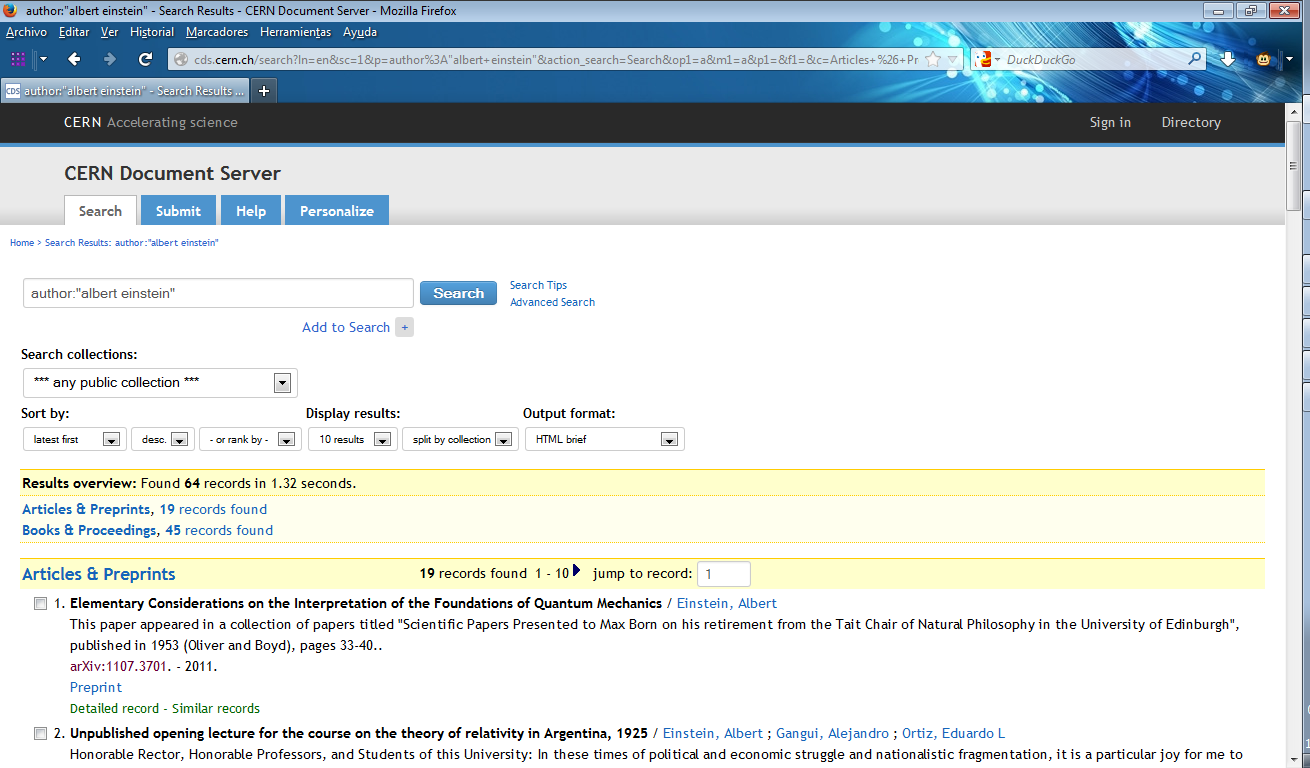
\includegraphics[height=3 cm]{images/figures/cds_screenshot.png}
\label{cds_screenshot}
\caption{CDS search result interface}
\end{figure}
 


Invenio\cite{invenio} is the open-source digital library software platform running behind CDS and it is a project developed in parallel to CDS at CERN. Besides CDS, Invenio supports around thirty scientific institutions worldwide including INSPIRE (a collaboration between Fermilab, CERN, DESY and SLAC) EPFL and ILO.
Invenio is composed of several modules, each one of which can be mapped to a specific step in the workflow of a record. Figure 1.2 presents the global architecture of Invenio. A detailed explanation of each module can be accessed in \cite{invenio_modules} 

\begin{figure}
\centering
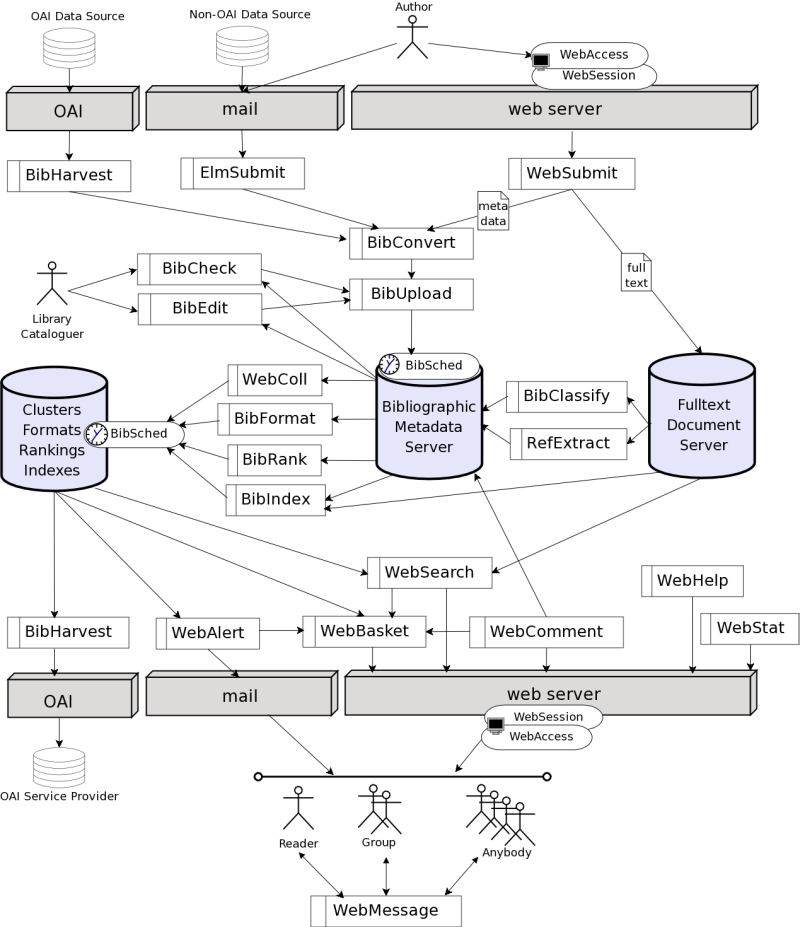
\includegraphics[height=4 cm]{images/figures/invenio.jpeg}
\label{invenio_architecture}
\caption{Invenio global architecture}
\end{figure}


\subsection{Project overview}
\subsection{Motivation}
The initial statement for this project was more generic and was encompassed as "New ways to programmatically, accurately and efficiently extract data and metadata from digital files". During a first exploration around this topic, we focused our attention to the mathematical content that is stored in these files. After more discussions we identified that the extraction, storage, indexing and finally searching for mathematical content would be a very useful project for CDS and an interesting research direction. CDS groups records in different categories or Collections such as Published Articles, Preprint, Photos, Books, General Talks among others. Some of these collections contain scientific documents in all of the different research areas where CERN is involved, and therefore a big amount of mathematical expressions are contained there. Only the Preprints collection contains 698581 records to date, harvesting documents from services like ArXiV\cite{arxiv} where most of the documents are in the areas of physics, mathematics and statistics which are very rich in mathematical content.
Currently Invenio provides different ways of searching for records by specifying metadata fields like author:"Albert Einstein" or by keywords. However, there is no way to search for a given mathematical expression. The current workarounds would be to try to search for the name of the given expression if it is common enough to have been named like \emph{Schr\"oodinger equation}. This approach most of the times is not enough since most of the equations are not named and even named ones can be rewritten in several ways and each one may have a different importance to the user. This combination of factors, motivates the development of a complete system that allows users to search for relevant documents, based on mathematical expressions.

\subsection{Goals}

The specific goals of this project can be summarized as:

\begin{itemize}
\item Explore ways to automatically extract the mathematical content from a document collection
\item Investigate different approaches and formats to store mathematical expressions
\item Identify relevant features in a mathematical expression 
\item Explore ways to efficiently store and retrieve the set of features
\item Implement the previous steps into a complete system (a search engine) and integrate it into the Invenio software
\item Evaluate different approaches and the quality of the provided results
\item Identify deficiencies in our work and propose solutions and further directions
\end{itemize}

\section{Related Work}
\subsection{Status of Mathematical Information Retrieval}
Even though Information Retrieval has been a research field from around the 1950s where the first metrics for such systems were developed and in the 1960s where SMART (System for Mechanical Analysis and Retrieval of Text), the first computer based system was developed; only in the last couple years focus have been put into adapting the same techniques to mathematical content. 

The Mathematics Information Retrieval Workshop\cite{mir_workshop} held in the context of the Conference of Intelligent Computer Mathematics in July 2012, was the first official event in the area of MIR. Here, a small competition was held to evaluate different systems and approaches.

The NII\cite{nii} (National Institute of Informatics) is a Japanese research institute that hosts the project named NTCIR (NII Testbeds and Community for Information access Research) which aims to build evaluation frameworks for specific sub-fields of information retrieval. On 2013, in the context of the 10th NTCIR conference, it hosted the NTCIR-10 Math Task \cite{math_task} which was the first collaborative effort to evaluate different systems. The Math task was focused on two different subtasks: Math retrieval (Identifying relevant document based on given mathematical expressions and/or keywords) and Math understanding where the idea was to extract natural language information of a mathematical expression in a document. Currently submissions are open for the NTCIR-11 Math Task 2 which will be held on December 2014.

\subsection{Mathematical based search projects}

\subsection{MIaS}
MIaS\cite{mias_1} (Math Indexer and Searcher), currently, is one of the flagship projects in the indexing and searching of mathematical content. As most of the other projects, it processes documents in MathML format. It allows the user to include in the queries mathematical expressions and textual content. During indexing time, equations are transformed following a set of heuristics that include:
\begin{itemize}
  \item Ordering of elements: Taking into account commutativity of certain operators (Addition, multiplication), elements are ordered such that $3 + a$ would be converted into $a + 3$ (Since the <mi> tag comes first than the <mn> tag)
  \item Unification of variables: This process takes into the account the structure of the equations in despite of the naming of the variables. Expressions like $a+b^a$ and $x+y^x$ would be converted into an expressions of the form $id_1 + id_2^{id_1}$ which would match.
  \item Unification of constants: This step consists of replacing all occurrences of constants (<mn> tags) by a const symbol. 
\end{itemize}
The extracted tokens from a given equation consist of all its valid sub-expressions. The original expression is given a weight value of 1, and following sub-expressions are given smaller weights depending on how general or specific they are.  
The system, also as most of the current projects, is developed by using the Apache Lucene framework. The system adapts the default scoring equation such that the given weight is taken into account.  
Publicly available instances of the system can be found at: \url{http://aura.fi.muni.cz:8085/webmias/ps?n=-1} running on the MREC\cite{mrec} dataset and  \url{ http://aura.fi.muni.cz:8085/webmias-ntcir/} (Running on the NTCIR dataset)

\subsection{EgoMath}
EgoMath\cite{egomath1} and its new version EgoMath$^2$\cite{egomath2}, is a system oriented to index the mathematical content from the Wikipedia.org database. The processing steps before indexing are similar to the ones in MIaS (Rearranging of symbols, unification of constants). The extraction process started from a complete dump of the Wikipedia database and filtering only the math articles, which are identified by the ”<math>" tag. This consists on around thirty thousand articles, from which 240.000 equations were identified. The processing step includes translating the equation from LaTeX into MathML format and then indexing both representation.
Some additional effort is done into splitting large mathematical blocks like tables into single mathematical expressions. At the start of this work, EgoMath was publicly available at \url{http://egomath.projekty.ms.mff.cuni.cz/}, however at this moment the system seems to be unavailable.

\subsection{DLMFSearch}
The Digital Library for Mathematical Funtions \cite{dlmf} is a project launched by the National Institute of Standards and Technology, in 2010, as an online version of the  Handbook of Mathematical Functions with Formulas, Graphs and Mathematical Tables\cite{handbook}. DLMF's main goal is to compile the mathematical knowledge in the form of equations, functions, tables and make this information useful for researchers and public in general. The system contains a search functionality that allows to input a combination of full text and \LaTeX snippets. The system tries to perform an exact match, and if no results are found, it relaxes the query. DLMF also perfoms some normalization of the equation and some cleaning of some characters, but no further details are provided. The content indexed by this project is highly curated, which differentiates it from the other projects. In the report published in 2013 \cite{dlmf2}, it is reported to have indexed around 38000 equations. This project is publicly available at \url{http://dlmf.nist.gov/}

\subsection{MathWebSearch}
MathWebSearch\cite{mathwebsearch} (Currently on its 0.5 version) is a open-source search engine for mathematical equations. While most of the documentation relates on the architecture of the system and how they address scalability; the indexing technique is also very interesting. The system implements and idea proposed by Peter Graf in \cite{substitution_tree_indexing} called substitution tree indexing. This idea can be viewed as a generalization of the variable and constant unification. It represents the equations as a tree an recursively generalizes each sub-expression. A public available instance of the system is available at \url{http://search.mathweb.org/tema/} which runs on the Zentralblatt Math database\cite{zb}.


\subsection{LaTeXSearch}
LaTeXSearch \url{http://latexsearch.com/} is a system developed by the scientific publisher Springer that allows to search over a database of around eight million latex snippets extracted from their publications. The system, unfortunately, is proprietary and no further details are provided.

\subsection{WikiMirs}
WikiMirs\cite{wikimirs} is a system that, as EgoMath, allows to find relevant Wikipedia entries by providing mathematical expression in \LaTeX. It combines the information about the semantic tree with the layout tree of a given expression and uses a similar approach to index different generalization levels. The system is available at \url{http://www.icst.pku.edu.cn/cpdp/wikimirs/} \\


Other systems that provide similar search functionalities are Uniquation(\url{http://uniquation.com}) and Symbolab(\url{http://www.symbolab.com/}), however detailed information about the systems are not provided. Finally Wolfram Alpha\cite{wolframalpha} is a very powerful tool that allows to find information about lots of mathematical concepts and a wide variety of other objects (Even Pokemon).


\section{$5e^{x+y}$(CDS)}
\label{chapter-cern_math_explorer}
In this chapter we present our solution called $5e^{x+y}$(CDS). We present the key points of our system, and how they are related to previous built systems.

\subsection{Features Extraction}
Our main goal is to develop a system that compliments the already available search capabilities in Invenio and in particular the CDS instance. Our system was developed on top of the  the Apache Lucene/Solr framework. CDS already uses Solr as a search engine layer, so developing $5e^{x+y}$(CDS) using this technology supposed a reasonable choice. One of the main steps while building an IR tool, is understanding the data and what kind of features can be extracted from it: If the system is based on text, then tasks such as stemming, handling of synonyms, misspelling and so on, should be taken into consideration; if the system being developed is based on images, then examples of features can be histograms of colors, geometrical features and so on. During the literature review, we discovered that most of the projects handled the notational aspects of the expressions, that is, the real naming of the terms in a given equation and each project developed its own set of heuristics to handle the structural component. 


\subsection{Notational Features}
Notational features correspond to the elements that relate to the actual naming of the variables, constants and numeric quantities found in an equation. Here we extract tokens that represent single leaf nodes (E.g. <mi>, <mn>, <mo> tags), and simple constructs like subscript and superscript elements, fractions, roots.
We also extract bi-grams and tri-grams as an analogy to what is done for text indexing in current systems.

After examining a set of documents from our dataset, we identified some heuristics that could be applied to improve the recall of our system:

\subsubsection{Unicode Normalizing} 
The first issue we discovered is that because of the wide range of different characters to represent the possible mathematical symbols, there is need for an automatic way to match different possible variations of a single character. An example of this situation is the specification of an natural number, sometimes denoted by the letter N. In this case, at least three different common representations were identified: $ N = 1 $ (Using character with unicode code point 0x004e), $\mathcal{N} = 1$ (0xd835 0xdc41 or in latex expressed as \lstinline|\mathcal{N}|) and $\mathbb{N} = 1$ (0x2115 or in latex expressed as \lstinline|\mathbb{N}|). \\
  To address this situation, we rely on the Unicode equivalence framework. In the unicode specification, sometimes the same character has two or more different code-points because of backwards compatibility with other encoding standards or because the same character has different essential meanings. Another group of equal characters with different code-points are pre-combined characters such as the Latin letter \~{N} which has Unicode point 0x00D1 and also is the sequence of code-points 0x004E (Latin letter N) and 0x0303 (the combining character tilde). Taking this sample into account, Unicode defines the character composition and decomposition operations as replacing the decomposed representation with the pre-composed one and vice-versa. Finally, Unicode defines two types of equivalences between characters: Canonical and compatible. Canonical equivalent characters are assumed to have the same appearance and meaning. Compatible ones are allowed to have slightly different graphical representations but the same meaning in some contexts. One example of compatible equivalent characters is the Roman number 12 {\unicodefontⅫ} with code-point 0x216b and the sequence of characters XII with codepoints 0x0058 0x0049 0x0049. Taking into account the composition or decomposition of characters and the canonical or compatible equivalences, Unicode specifies 4 different forms of a given character:
  \begin{itemize}
  \itemsep0em
  \item NFD: Normalization Form Canonical Decomposition
  \item NFC: Normalization Form Canonical Composition
  \item NFKD: Normalization Form Compatibility Decomposition
  \item NFKC: Normalization Form Compatibility Composition
  \end{itemize}
  
Table \ref{unicode_characters} presents a small list of troubling characters classes that were identified in our datasets.



Since our goal is to match as many similar characters as possible, our system employs the NFKD representation of a character. For a given token, we test whether if it is already equal to its NFKD. If not, for all the characters that are not combining nor control characters, we add the token into the same position as the original one.
For example, given the token <mi>\r{A}</mi>, this will lead to the sequence <mi>\r{A}</mi><mi>A</mi> and the token <mi>{\unicodefontⅫ}</mi> will produce <mi>{\unicodefontⅫ}</mi><mi>X</mi><mi>I</mi><mi>I</mi>.

\subsubsection{Operator grouping}
Even though the Unicode normalization step works for a big part of the cases presented in table \ref{unicode_characters}, there are still some groups of characters which would not be matched (even partially), such as some types of integrals. To address these groups, a precomputed table was created for some general groups of operators which have some similar meaning. For each token that belongs to some of this predefined groups, a second token is created identifying the group.
For example the token <mo>{\unicodefont ∮}</mo> is expanded into <mo>{\unicodefont ∮}</mo> <mo>INTEGRALS</mo>, similarly the token <mo>{\unicodefont ∫}</mo> is expanded into <mo>{\unicodefont ∫}</mo> <mo>INTEGRALS</mo> and then both will have a partial match in the INTEGRALS token. 
The Unicode specification does not define a strict rule to group similar characters based on their semantics. For general operators, we used the grouping provided by Xah Lee in his website\cite{math_groups}.

Figures \ref{integrals} and \ref{less_greater} present lists related of characters for two different categories.

\begin{figure}[h!]
	\centering
	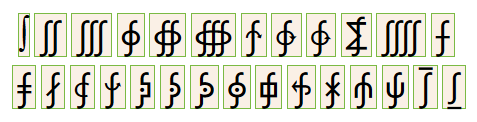
\includegraphics[height=2 cm]{images/figures/integrals.png}
	\caption{List of different types of integral related characters in Unicode}
	\label{integrals}
\end{figure}

\begin{figure}[h!]
	\centering
	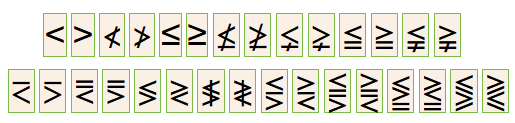
\includegraphics[height=2 cm]{images/figures/greater_less.png}
	\caption{List of different types of greater/less than related characters in Unicode}
	\label{less_greater}
\end{figure}

\subsubsection{Numeric Approximation} 
Some equations relate to specific numeric quantities. While most of the previously explorer systems handled <mn> tags by only representing them as a constant identifier, this approach is not suitable. A lot of articles in CDS relate to specific experiments under certain conditions, and require a high level of precision in the measurements. However, different experiments of the same phenomenon, can result in different measurements and we wanted to include this variability in our system. To handle this, when a token with a certain numeric quantity is discovered, we apply iterative rounding and index all the different approximations in the same position as the original element. For example the token <mn>2.0135</mn> will produce the following sequence of tokens: <mn>2.0135</mn><mn>2.014</mn><mn>2.01</mn><mn>2.0</mn>. 


\subsection{Structural Features}
The structure of a mathematical expression compliments the information that can be obtained over generic substructures where the naming of the variables is irrelevant.  

\subsubsection{Algebraic structures}
The first set of structures consists of purely algebraic relationships between the expressions.
Inspired by predefined integral tables for different kinds of expressions, we decided to extract, from a given equation, whether it has an occurrence of these kinds of patterns or not.
An example of this type of structures would be: $X\textunderscore*(X\textunderscore + A\textunderscore)$ where $X\textunderscore$ and $A\textunderscore$ can be any type of expression. Sample equations matching this pattern can be $C (C+1)$ or $\frac{(\sin{\theta}\cos{\theta})^2}{2a} (\frac{(\sin{\theta}\cos{\theta})^2}{2a} + \tan{\frac{\theta+\phi}{2}})$. This structural analysis of equations is more powerful than the unification of variables and constants proposed in previously discussed projects because these patterns, as shown in the second example, can match an arbitrary complex expression. The drawback of our solution is the need to manually select representative and useful patterns. This selection was done based on standard based tables of integrals similar to the ones that CASs employ to compute them.

\subsubsection{Subscript/Superscript variations}
This set of structures represent common operations that can appear in a given expression, but its identification is based on notation factors. A simple example of this can be the matrix decomposition $A = VDV^{-1}$ where the actual name of the variables $A$ and $V$ is not meaningful but the real importance is the fact that a given variable appears alongside its inverse in a matrix multiplication form. We would like to assign a partial match to any other kind of this decomposition say $B = MRM^{-1}$. These types of structures live in-between the notational and structural categories but since we identify them using Mathematica, we encompass them as structural features. For this type of structures, we identify simple operations between an element and some possible variations of the same element with some subscript/superscript.

\subsubsection{Specific domain structures}

Additionally, there are common patterns to specific domains which can improve the quality of the retrieved results. Some specific patterns we identified include: $originalParticle \rightarrow subparticle1, subparticle2, subparticle3$ (for representing particle decaying processes) $S = \int^{t2}_{t1} \mathcal{L} dt$ (for an action in terms of its Lagrangian) and $SU(n)$ (for describing special unitary groups). The main drawback of this approach is the need to manually detect, implement and maintain long lists of patterns and for this reason we did not try to assemble an exhaustive list.


\section{Development with Lucene/Solr}
This section explains how the described components were implemented in the {\codefont Apache Lucene/Solr} framework.
One focus of our work was to develop a modular system that allowed easily to deploy new heuristics as they were identified. 

The Lucene framework defines some key concepts which ultimately are mapped into concrete classes. A {\codefont Document} is the minimum retrieval unit. For $5e^{x+y}$ we could either use a complete article as a document or a single equation. We choose the latter because it makes it easier to focus on extracting features from a single equation. A document contains a set of {\codefont fields} which represent different types of information that it can store. Each field has different options such as whether it would be indexed and/or stored. A field can also indicate whether it will be a {\codefont Term Vector}. Our fields are as follow: 
\begin{itemize}
\item math\_notational\_field: This field stores the notational features as a Term Vector. 
\item math\_structural\_field: This field stores the structural features as a Term Vector. 
\item math\_normalized\_notational\_field: This field stores the notational features of the normalized expression as a Term Vector. 
\item filename: This is an auxiliary field which stores the CDS record / article name where the equation was found.
\item number\_occurrences: Another auxiliary field that is used to score final results.
\end{itemize} 

Each field is associated to a particular {\codefont Analyzer}. An analyzer is a specific class that handles an element from a field and groups all the operations that are to be performed. For this purpose we implemented {\codefont SolrNotationalAnalyzer}, {\codefont SolrStructuralAnalyzer} and {\codefont SolrNormalizedNotationalAnalyzer}. 
The Solr prefix is added to clarify the fact that the class extends a {\codefont SolrAnalyzer} which extends a normal lucene {\codefont Analyzer}. 

An analyzer consists of a sequence of {\codefont TokenStrem} elements. Normally an analyzer contains one {\codefont Tokenizer} element (which extends a {\codefont TokenStrem}) that is in charge of creating the Terms that will be stored in the field, and one or more {\codefont TokenFilter} elements which perform operations on the single tokens that were created previously. For the specific cases of SolrNotationalAnalyzer and SolrNormalizedNotationalAnalyzer we created the following classes: 

\begin{itemize}
\item {\codefont MultiplePatternTokenizer}: This class is in charge of applying a set of regular expressions over the given expression in order to extract the single elements that were presented. Lucene incorporates the class {\codefont PatternTokenizer} but it only accepts one regular expression.
\item {\codefont UnicodeNormalizingFilter}: This class receives single tokens and verifies if the token is in Unicode NFKD. In negative case, it emits an additional token in the normalized form.
\item {\codefont SynonymExpandingFilter}: This class verifies if the received token belongs to a predefined category of elements and emits an additional token with it.
\item {\codefont NumericalRoundingFilter}: This class processes {\codefont <mn>} tokens. When a number contains a decimal part, it applies the standard rounding mode iteratively and for each one, it emits a token for each step. 
\end{itemize}

{\codefont SolrStructuralAnalyzer } is simpler in its workflow: It consits of a {\codefont StructuralPatternsTokenizer} that tries to find occurrences of the predefined patterns in the expression. For each match, it emits a token with the pattern that was found. 

\subsection{Integration with Mathematica}
This section describes some aspects that had to be considered while implementing the integration with Mathematica. Our system uses the {\codefont JLink} library to create a connection with the underlying process {\codefont MathKernel}. The main class for communicating java code and {\codefont Mathematica} is {\codefont KernelLink} and the main used method was {\codefont evaluateToOutputForm(String expr, int pageWidth)} where {\codefont expr} is the expression to be evaluated and {\codefont pageWidth} affects the formatting of the result.
Once all the boilerplate has been written, the steps followed to define and find patterns in the expression are as follow: We import the string in MathML format through the command {\codefont ImportString["<mathmlExpression>", "MathML"]}. This creates the expression in the box form, but no further analysis is possible from this form. We then try to interpret this form into a fully Mathematica compatible expression by using {\codefont MakeExpression}


\subsection{Pattern Extraction}
Once the expression is created, finding a pattern is easy by using the command {\codefont Position[<variable holding the interpreted expression> , Pattern]}. A simple pattern for a quadratic expression is: {\codefont a\_.x\^{} 2 + b\_.x + c\_.} 

\subsection{Cleaning of variables}
After each operation, all of the variables should be cleaned or it may lead to deadlocks, wrong results or other issues since the {\codefont MakeExpression} command also interprets the expression so if the expression is, for example {\codefont a = b + c} Mathematica remembers the assignment of the new value of {\codefont a} and uses it in further evaluations. The cleaning is done through the command {\codefont Remove["Global`*"]}


\subsection{Expression simplification}
The second feature that we are interested in is automatic expression simplification.
Mathematica includes different transformations of expressions. These include: {\codefont Simplify} which tries to transform a given equation in an equivalent one but in a reduced form, {\codefont FullSimplify} which is similar to the previous one but tries a higher number of heuristics to apply that can simplify expressions further at the expense of more processing time, {\codefont Factor} to factorize polynomials, {\codefont Refine} which simplifies expressions given certain assumptions about the variables, {\codefont TrigReduce} that tries to apply trigonometric identities to simplify the expression, {\codefont FunctionExpand} that tries to expand special functions in terms of sums and products of other elementary functions. 

The two functions that are more relevant for our work are {\codefont Simplify} and {\codefont FullySimplify} since they apply a combination of the other methods and do not require additional information.

Table \ref{comparison_simplification} presents some sample equations found in some the documents in CDS and the different forms of simplification.



\subsection{Recursive interpretation}
Unfortunately, Mathematica cannot always interpret correctly an input expression. In this case, it can, however interpret some sub-expressions from the original one. Our system takes advantage of this, and the first attempt is to try to interpret the original string. If this step is not successful (the result variable equals the string "\{\}"), we identify the occurrences of {\codefont RowBox} which identify all the subexpressions in the tree. For each of this elements we call the {\codefont MakeExpression} and if it was successful we search for structural patterns in it. A first thought would tell us that if sub-tree was interpreted successfully, there is no need to try to go further down in that sub-tree, however, even if a sub-expression is interpreted correctly, the result sometimes is not complete and processing further down gives better results. For this reason, we do not discard any of the subexpressions and try to interpret all of them. For this same reason, we do not store the number of occurrences of a given pattern, but only whether it contains is or not.

\subsection{Error handling}
Sometimes, after certain time, the connection between {\codefont KernelLink} and {\codefont Mathematica} is lost and it launches an exception and all following invocations fail as well.
Also, re-instantiating a KernelLink would yield an Exception. For this scenario, killing the associated processes to Mathematica was necessary with {\codefont killall -s 9 Mathematica; killall -s 9 MathKernel
} or {\codefont taskkill /im Mathematica.exe; taskkill /im MathKernel.exe} depending on the OS the system is running on.

With this, the next creation of a new KernelLink works properly and the subsequent invocations work as expected.


\subsection{Timeout Handling}
Unfortunately, checking the quality of a LaTeX document is a difficult job and users have a lot of freedom in the way they write their document since the only visible result is the rendered version. 
One example we found during our work is the following TeX snippet:
\begin{verbatim}
	"\ \varphi\ are\ shown,\ as\ well\ as\ the\ weight\ and\ tension"
\end{verbatim}
A human can easily identify that this corresponds to text and that should be inserted into a proper "mbox" or "text" tag. In this case, the snippet produced the following MathML code:
\small{\codefont <math><mrow><mi>φ</mi><mo></mo><mrow><mi>a</mi><mo></mo>
<mi>r</mi><mo></mo><mi>e</mi></mrow><mo></mo><mrow><mi>s
</mi><mo></mo><mi>h</mi><mo></mo><mi>o</mi><mo></mo><mi>
w</mi><mo></mo><mi>n</mi></mrow><mo>,</mo><mrow><mi>a</m
i><mo></mo><mi>s</mi></mrow><mo></mo><mrow><mi>w</mi><mo
></mo><mi>e</mi><mo></mo><mi>l</mi><mo></mo><mi>l</mi></
mrow><mo></mo><mrow><mi>a</mi><mo></mo><mi>s</mi></mrow>
<mo></mo><mrow><mi>t</mi><mo></mo><mi>h</mi><mo></mo><mi
>e</mi></mrow><mo></mo><mrow><mi>w</mi><mo></mo><mi>e</m
i><mo></mo><mi>i</mi><mo></mo><mi>g</mi><mo></mo><mi>h</
mi><mo></mo><mi>t</mi></mrow><mo></mo><mrow><mi>a</mi><m
o></mo><mi>n</mi><mo></mo><mi>d</mi></mrow><mo></mo><mro
w><mi>t</mi><mo></mo><mi>e</mi><mo></mo><mi>n</mi><mo></
mo><mi>s</mi><mo></mo><mi>i</mi><mo></mo><mi>o</mi><mo><
/mo><mi>n</mi></mrow></mrow></math>
}

Mathematica took around 10 minutes to interpret it.
In the ideal case we would be able to identify the malformed expressions and pass to Mathematica only well-formed equations to be processed but as this simple example shows, that is a very challenging task and may require more work.
As a remedial situation, we used a fixed timeout to stop the processing of such expressions.

\section{Integration with CDS}
Currently the Invenio code-base is being under a deep refactoring and rewriting. CDS currently runs in the stable branch {\codefont master} while the new developments are preferred to be implemented in the new branch {\codefont pu}. 
Our system is deployed as a standalone {\codefont jar} which is added to a Solr instance. Also, some extra configurations should be added. Details on this can be found in appendix \ref{appendix-conf_files}.
The communication between Solr and Invenio was through the library {\codefont solrpy}. 
Figure 5.3 presents the main components of our deployment.

\begin{figure}[h!]
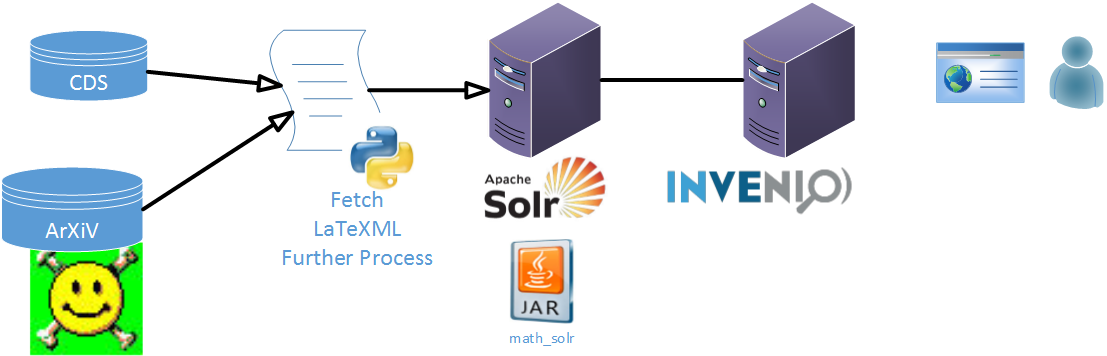
\includegraphics[height=3 cm]{images/visio_drawings/architecture.png}
\label{system_arch}
\caption{High level deployment architecture}
\end{figure}


A demo interface over the {\codefont pu} branch was developed to showcase the system, however to have a complete integration with CDS, more work is required. The demo setup employs the same dataset as used for experimentation.
We include an online \LaTeX\ editor\cite{latex_editor} that renders the input expression as the user types it. 

\begin{figure}
\center
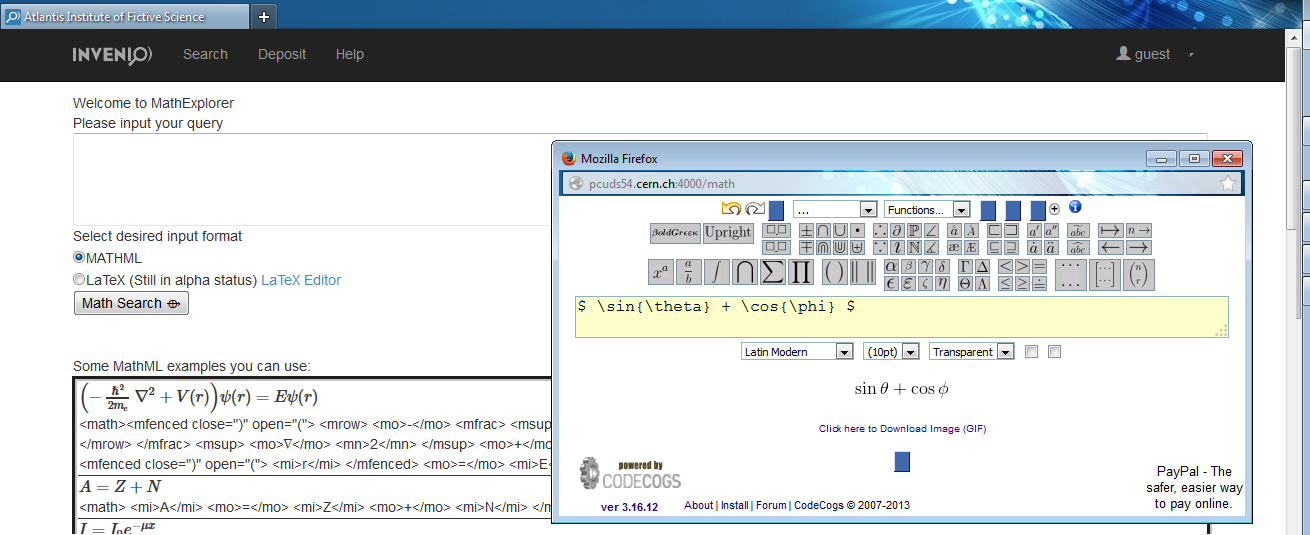
\includegraphics[height=3 cm]{images/figures/input_interface.png}
\label{input_int}
\caption{Web interface of $5e^{x+y}$: Query input screen}
\end{figure}

\begin{figure}
\center
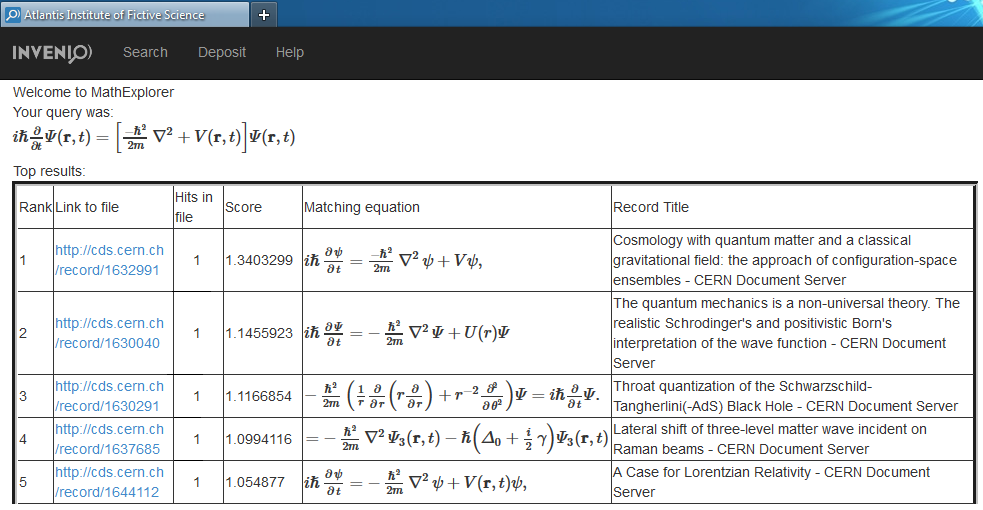
\includegraphics[height=3 cm]{images/figures/results_interface.png}
\label{results_int}
\caption{Web interface of $5e^{x+y}$: Results screen}
\end{figure}
	
 

\section{Evaluation}
When building an IR system there are two main aspects that should be considered. One is the quality of the presented results and the second one is the performance of the system since web users currently tolerate some milliseconds of latency for retrieving results. 

\subsection{Dataset}
Our dataset consists on 12234 latex documents fetched from ArXiV. This documents correspond to the latest records harvested for CDS. The documents were processed using LateXML as described in the extraction process. From the given dataset, the simpler equations were filtered out (The ones containing one or two elements). The total number of indexed equations is 1412297.

\subsection{Setup}

The machine used for experiments has a Intel Core i7 processor running at 3.4Ghz with 4 cores. The available RAM is 8Gb, and the Java Virtual Machine used for running Solr was run with the {\codefont -Xms2G -Xmx5G} parameters. The complete specifications of the used software is presented in table \ref{sw_used}



\section{Quality results}
In this section we are interested in evaluating the quality of the results provided by our system.
The type of queries that $5e^{x+y}$ was designed for, are typical equations that can be found in a physics scientific publication. 
Our main user case is that a user of CDS is interested in finding documents inside the collection whose equations are related to the one that is provided.  

The evaluated queries were provided by physics experts working at CERN from their own research topics. The queries were provided in \LaTeX\ format as the users used them in their own publications.
Table \ref{equations_table} presents the set of queries that were evaluated, and a simple explanation about each one. 
Each of the users evaluated the results only for the equations he/she provided. For each of the presented result, the user ranked it as "Strictly Relevant", "Partially Relevant" and "Completely Irrelevant". As all evaluations including human interaction, this scoring is at some level subjective. 

For each metric we compared three different scenarios:

\begin{itemize}
\item N : Only notational features over the original expression were used
\item N+S : Notational and structural features over the original expression
\item N+S+NN : Notational and structural features over the original expression and notational features over the normalized string using Mathematica's Simplify function
\item N+S+NN (BM25): Same scenario as before but using BM25 similarity function instead of TF-IDF. This scoring function is implemented in Lucene through the class {\codefont BM25Similarity}
\end{itemize}

We also were interested in also using the Fully Simplify function in Mathematica but we found no difference between both forms and the results were the same.

We present results for three metrics: Partial precision (Document either partially relevant or completely relevant) strict precision and discounted cumulative gain ($ \mathrm{DCG_{p}} = \sum_{i=1}^{p} \frac{ 2^{rel_{i}} - 1 }{ \log_{2}(i+1)} $) which measures, in addition, the order of the results..






Results show that for the selected queries, the system performs reasonably well achieving a precision of 0.84 in the top 5 results in the best scenario and 0.65 in the top 20 results. 
Even more important than the absolute values, it is more interesting to see how the addition of structural features and the addition of normalization to the expressions, allows the system to improve its performance reasonably. In the top 20 results there was an increase of 15\% from the N scenario to the N+S+NN one. Also we see that in the case of the top 5 results going from N+S to N+S+NN resulted in the same strict precision of 0.84, it still represented and increase in the DCG metric which means still results were improved. 
A final remark is that there was not a significant difference between the two different similarity functions that were evaluated, and in at least one case, BM25 performed worse than standard tf-idf. 

\subsection{Indexing Performance}
For this set of evaluations, we were only interested in observing how the performance of the indexing stage is affected by the different types of features that are employed. We selected the first 100 records from our dataset and measured the total time it required to index all the elements in Solr using a python script and the solrpy library to do the communication. The default similarity in Solr was used. We also measured the index size at the end of each experiment.
Our four scenarios were organized as follows:
We tested the same three scenarios as for the quality results and we added a fourth one N+S+FN where we used the fully normalized form of the expressions as opposed to the standard simplified form in the N+S+NN scenario.

Table \ref{indexing_performance} summarizes the results of this set of experiments. The first result is the significant increase in processing time when using Mathematica. Going from the N scenario to N+S represent an increase of almost 15x in the indexing time. Adding standard normalization increases the indexing time by a factor near to 1.44x and full normalization by a factor of 1.55x.

With respect to storage size, we see a small footprint (Less than 5\%)in the total size by going from N to N+S. Adding normalization represents an increase by a factor of 1.78x and the size of the fully normalized index represents a smaller increase (1.76x)

We can observe that there is a small trade-off between time and storage size depending on which normalization mode is employed.



\subsection{Querying Performance}
Similarly, we were also interested in evaluating how the query performance of the queries was affected with the different scenarios. For this set of queries we used the complete dataset, and evaluated the N and the N+S+NN scenarios for queries of different length.


Table \ref{query_performance} shows that for smaller queries, the querying time increases from an average of 0.178 seconds to 0.327 which represents an increase of 83\%. For the largest evaluated set of queries, the querying time passed from 0.393 to 2.066 seconds which represents an increase of around 425\%. The absolute values, however, show that in the worst case the slower query took a little more than 2 seconds in average which is still acceptable for a specialized search engine.

\subsection{Alternative Metrics}
According to some experimental evaluations presented in \cite{tree_comparison}, Tree Edit Distance provides an interesting alternative metric to the standard vector space model using angular distance. In this work, authors present an improvement in the quality of retrieved results compared to the classic approach of indexing the single leaves of the tree and a subset of the possible sub-trees. For evaluating the feasibility of this approach we compared a set of equations using both metrics: Tree edit distance (Using Zheng and Shasha's algorithm implemented in python \cite{tree_distance_python}.) and a standard angular distance that was not heavily optimized. We compared elapsed times for expressions of different length.


This result show that for shorter expressions, using tree edit distance represent an increase in time in more than 200x, and a factor of around 1200x for the longer expressions, making it impractical for implementing a system that needs to be responsive. Even though there are algorithms which provide a better asymptotic guarantees and better actual running times like RTED\cite{rted} with respect to Zheng ans Shasha's algorithm, the best improvements represent a decrease in processing time of 50\% to 80\% in trees with around 1000 nodes, while the standard tested equations which are representative of our dataset, contain less than 100 nodes.
\section{Conclusions}
\label{chap-conclusions}

The area of Mathematical Information Retrieval (MIR) is still very young and different systems, algorithms and datasets are being developed. Our work, $5e^{x+y}$, proposes a complete MIR system for a concrete digital library, such as the CERN Document Server based on the Invenio digital library software platform. In terms of our proposed goals we can conclude that:

\begin{itemize}
\item We explored and identified different tools and approaches to automatically detect and extract mathematical content from digital files. We concluded that LaTeXML and InftyReader are currently the most suitable set of tools to process Latex and PDF files respectively. We automatized the extraction process and incorporated it into the Invenio workflow.
\item Our exploration of the extraction tools, lead us to identify the MathML format as the best format to store and process mathematical content. It is the recommended language for web documents, and the best extraction tools agree on it.
\item Once a mathematical expression is extracted and parsed to a suitable format the next step is to identify suitable features to index. We separated our features into notational and structural ones. For the first category, we discovered  some issues that have not yet been addressed in previous work and developed heuristics that allow to match more cases by normalizing unicode characters, grouping similar operators and expanding different numeric quantities. For the structural features, we explored the integration of a Computer Algebra System  to perform pattern matching and simplification of the given expression. 
\item We explored different IR frameworks and models to store and retrieve the indexed expressions and found that the standard vector space model is suitable for our needs.  
\item We implemented our system in top of the Lucene/Solr framework. We took advantage of the modular design of Lucene to structure our work in independent classes where each one has a defined role. This structure also allows to easily implement and incorporate further heuristics to handle more cases. Our system is deployed as a Solr plugin making it very easy to be used from an external application. As a final component in our system, we developed the glue code to integrate our search engine with Invenio and developed a simple web interface.
\item We performed different sets of evaluation on our system to explore the quality of the retrieved results and the performance of our system. Our quality evaluations showed that a combination of notational and structural features allow us to achieve significantly better results. Our performance results showed that the extraction of structural features through the Mathematica CAS imposes a heavy overhead of more than 10x on the indexing time, but as discussed previously, the extra work is worth investing in, given the improved set of results. The extra overhead at querying time is not insignificant but it is still acceptable for today's web usage standards. Our evaluation discarded the tree edit distance because the running time was 200 times more than the time needed by a simple angular distance used in standard vector space model implementations, making this approach impractical for a big system.
\item Finally, during this work we identified areas of improvement which are worth looking into. They are presented in the next chapter.
\end{itemize}




%ACKNOWLEDGMENTS are optional
\section{Acknowledgments}
We would like to thanks the ScienceWISE team for the help and important insights that they provided for the realization of this project.

%
% The following two commands are all you need in the
% initial runs of your .tex file to
% produce the bibliography for the citations in your paper.
\bibliographystyle{abbrv}
\bibliography{bibliography}  % sigproc.bib is the name of the Bibliography in this case
% You must have a proper ".bib" file
%  and remember to run:
% latex bibtex latex latex
% to resolve all references
%
% ACM needs 'a single self-contained file'!
%
%APPENDICES are optional
%\balancecolumns
\end{document}
